\section{Aufgaben}

\subsection{hello-world.cc}
\begin{frame}{Ziel}
 \begin{itemize}
  \item \cod{hello-world} auf dem \host und auf dem \targetS
  \item \cod{primes} auf dem \host und auf dem \targetS
 \end{itemize}
\end{frame}


\begin{frame}{The big Picture}
 \begin{itemize}
  \item Source File: \cod{hello-world.cc}
  \item falls es nicht klapt ?
  \begin{itemize}
   \item wo ist der File ?
  \end{itemize}
 \end{itemize}
\end{frame}

\subsection{Zugriff auf die Hardware}
\begin{frame}{Scripts}
 \begin{itemize}
  \item \cod{led-enable.sh}
  \item \cod{led-blink.sh}
 \end{itemize}
\end{frame}

\begin{frame}{C++}{mit \cod{/sys/class/gpio}}
 \begin{itemize}
  \item \cod{led-enable.cc}
  \item \cod{led-blink.cc}
 \end{itemize}
\end{frame}

\begin{frame}{C++}{direkt mit \cod{mem.h$|$cc}}
 \begin{itemize}
  \item \cod{led-direct-0.cc}
  \item \cod{led-direct-1.cc}
 \end{itemize}
\end{frame}

\subsection{Zugriff auf die andere Hardware}

\begin{frame}{Input \& Output}
 \begin{center}
  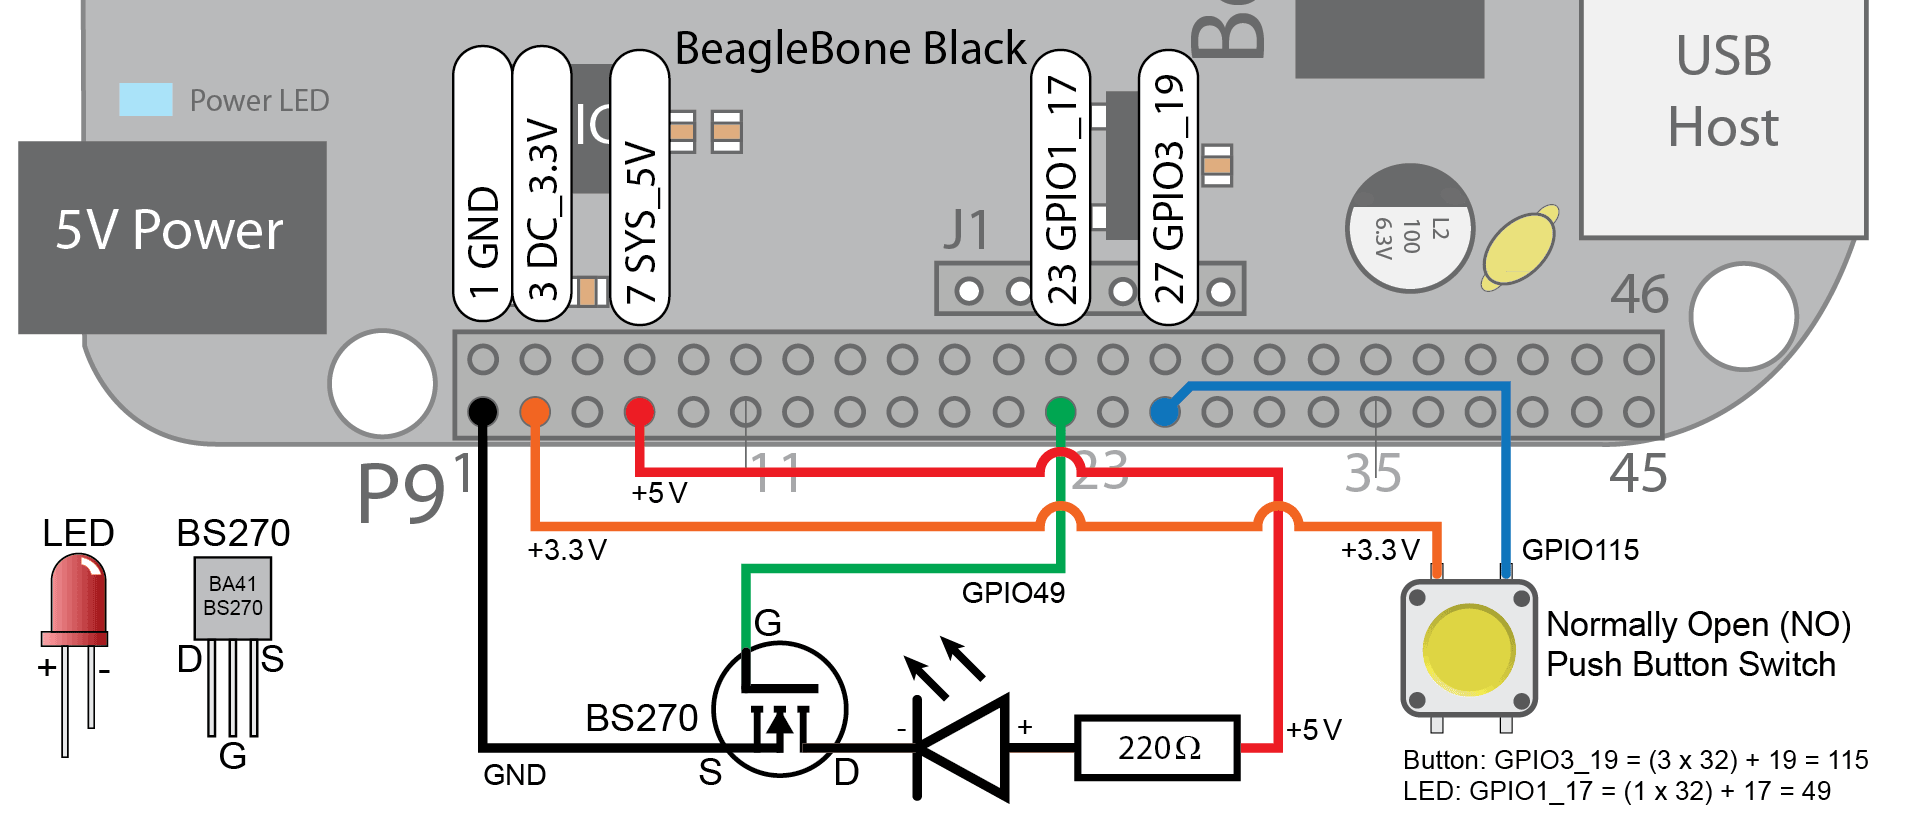
\includegraphics[width=0.875\textwidth]{Button-and-LED-large.png}
 \end{center}
 \begin{itemize}
  \item Output LED (Script,C++)
  \item Input SWITCH (Script,C++)
 \end{itemize}
\end{frame}

\begin{frame}{Input \& Output}{Kombination}
 \begin{itemize}
  \item SWITCH $\to$ LED
  \begin{itemize}
   \item Script
   \item C++
  \end{itemize}
 \end{itemize}
\end{frame}

\subsection{LED via Internet}

\begin{frame}{LED via Internet}{Was Sie brauchen}
\begin{itemize}
 \item die LED Hardware
 \item einen HTTP Server 
 \begin{itemize}
  \item \href{https://www.lighttpd.net/}{$\to$lighttpd}
  \item den Code finden Sie auf \href{https://drive.switch.ch/index.php/s/0MfVmFD4WAeJXvS}{$\to$lighthttpd.tar.xz}
 \end{itemize}
 \item Common Gateway Interface (CGI)
 \begin{itemize}
  \item \cod{src/cgi0.cc} für den ersten Test
  \item \cod{src/cgi.h/cc} das {\em framework}
  \item \cod{src/cgi-test.cc} gfür den Test von \cod{src/cgi.h/cc}
 \end{itemize}
 \item Die Verbindung zur Hardware
 \begin{itemize}
  \item \cod{src/gpio.h/cc}
 \end{itemize}
\end{itemize}
\end{frame}

\begin{frame}{Die Herstellung}
 \begin{itemize}
  \item \cod{lighttpd}
  \begin{itemize}
   \item Installation: \cod{lighthttpd.tar.xz}
   \item Konfiguration: \cod{config/lighttpd.conf}
  \end{itemize}
  \item CGI/GPIO (Makefile)
  \begin{itemize}
   \item \cod{src/cgi0.cc} für den ersten Test
   \item \cod{src/cgi.h/cc} das {\em framework}
   \item \cod{src/cgi-test.cc} gfür den Test von \cod{src/cgi.h/cc}
   \item \cod{src/gpio.h/cc}
  \end{itemize}
 \end{itemize}
\end{frame}
